\usetikzlibrary{arrows.meta,calc}
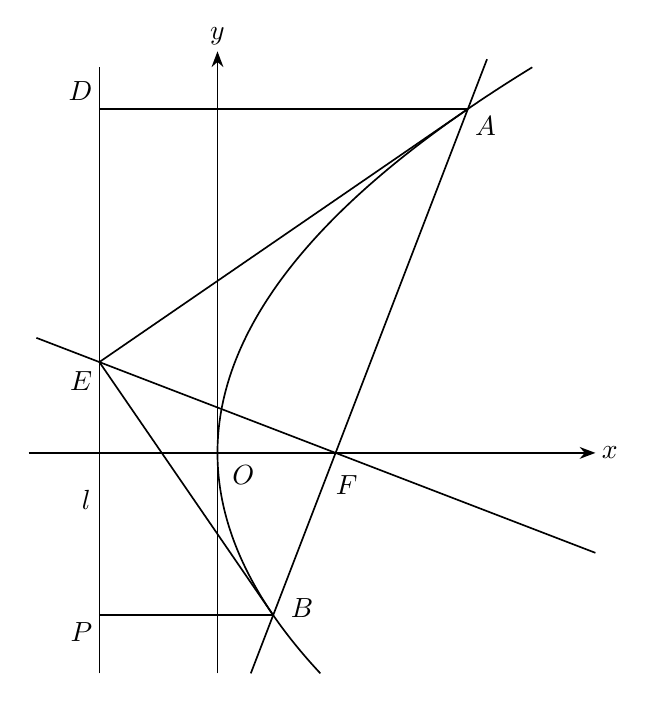
\begin{tikzpicture}[x=1cm,y=1cm,line width=.6pt,font=\normalsize,>=Stealth]
  \coordinate (O) at (0,0);
  \coordinate (F) at (1.5,0);
  \coordinate (A) at (3.1800344625,4.3680896024);
  \coordinate (B) at (0.7075395020,-2.0603972947);
  \coordinate (D) at (-1.5,4.3680896024);
  \coordinate (E) at (-1.5,1.1538461538);
  \coordinate (P) at (-1.5,-2.0603972947);
  \draw[->] (-2.4,0)--(4.8,0);
  \node[right=2pt,inner sep=0pt] at (4.8,0) {$x$};
  \draw[->] (0,-2.8)--(0,5.1);
  \node[above=2pt,inner sep=0pt] at (0,5.1) {$y$};
  \draw[line width=.6pt,samples=161,domain=-2.8:4.9] plot ({\x*\x/6},{\x});
  \draw (-1.5,-2.8)--(-1.5,4.9);
  \draw (D)--(A);
  \draw (P)--(B);
  \draw (E)--(A);
  \draw (E)--(B);
  \draw (0.4230769231,-2.8)--(3.4230769231,5.0);
  \draw (-2.3,1.4615384615)--(4.8,-1.2692307692);
  \node[anchor=south east,inner sep=0pt] at (-1.58,4.46) {$D$};
  \node[anchor=north west,inner sep=0pt] at (3.26,4.28) {$A$};
  \node[anchor=west,inner sep=0pt] at (0.92,-1.97) {$B$};
  \node[anchor=north east,inner sep=0pt] at (-1.58,1.04) {$E$};
  \node[anchor=north,inner sep=0pt] at (1.64,-0.28) {$F$};
  \node[anchor=north west,inner sep=0pt] at (0.18,-0.15) {$O$};
  \node[anchor=north east,inner sep=0pt] at (-1.58,-2.15) {$P$};
  \node[anchor=east,inner sep=0pt] at (-1.60,-0.60) {$l$};
\end{tikzpicture}
